% from Helmund slides
\documentclass[tikz,border=10pt]{standalone}
%\documentclass[crop, tikz]{standalone}

\usepackage{tikz}
\usetikzlibrary{calc,through}

\begin{document}

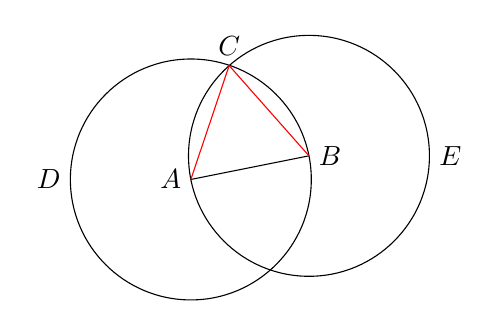
\begin{tikzpicture}[scale=1.2]
	% establish the coordinates for the master reference points
	\coordinate [label=left: $A$] (A) at (0, 0);
	\coordinate [label=right:$B$] (B) at (1.25, 0.25);
	
	% draw the geometries
	\draw (A) -- (B);   % line between A and B
	
	% Node D will be when we draw a circle at A (center) that passes through B
	\node (D) [draw, circle through=(B), label=left:$D$] at (A) {};
	% Node E will be when we draw a circle at B ( center) that passes through A
	\node (E) [draw, circle through=(A), label=right:$E$] at (B) {};
	
	\coordinate[label=above:$C$] (C) at (intersection 2 of D and E);
	
	\draw [red] (A) -- (C);
	\draw [red] (B) -- (C);

\end{tikzpicture}

\end{document}